\documentclass[a4paper,11pt,notitlepage]{report}
% Henrik Kramselund  , February 2001
% hlk@security6.net,
% My standard packages
\usepackage{zencurity-exercises}

\begin{document}

\rm
\selectlanguage{english}
\newcommand{\subject}[1]{Networking, TCP/IP and Security for Beginners workshop}
\mytitle{Networking, TCP/IP and Security for Beginners}{exercises}

\setcounter{tocdepth}{0}

{\color{titlecolor}
\renewcommand{\baselinestretch}{0.3}\setlength{\parskip}{1mm}
\tableofcontents}
%\listoffigures - not used
%\listoftables - not used

\normal
\pagestyle{fancyplain}
\chapter*{\color{titlecolor}Preface}
\markboth{Preface}{}

This material was originally prepared for use in a workshop \emph{Networking, TCP/IP and Security for Beginners} and was prepared by
Henrik Kramselund  , \link{http://www.zencurity.com} .
It describes the networking setup and
applications for trainings and workshops where hands-on exercises are needed.

Further a presentation is used which is available as PDF from kramse@Github\\
Look for \jobname\ in the repo security-courses.

These exercises are expected to be performed in a training setting with network connected systems. The exercises use a number of tools which can be copied and reused after training. A lot is described about setting up your workstation in the repo

\link{https://github.com/kramse/kramse-labs}

Dont be scared away by the many exercises, you can pick a few and have fun with those and ignore the rest. If you one day need to research network security the others may come in handy \smiley

The exercise list includes my recommended tools I use myself and for teaching.

\section*{\color{titlecolor}Prerequisites}

This material expect that participants have a working knowledge of
TCP/IP from a user perspective. Basic concepts such as web site addresses and email should be known as well as IP-addresses and common protocols like DHCP.


\vskip 1cm
Have fun and learn



\begin{figure}[H]
\label{fig:osi}
\begin{center}
\colorbox{white}{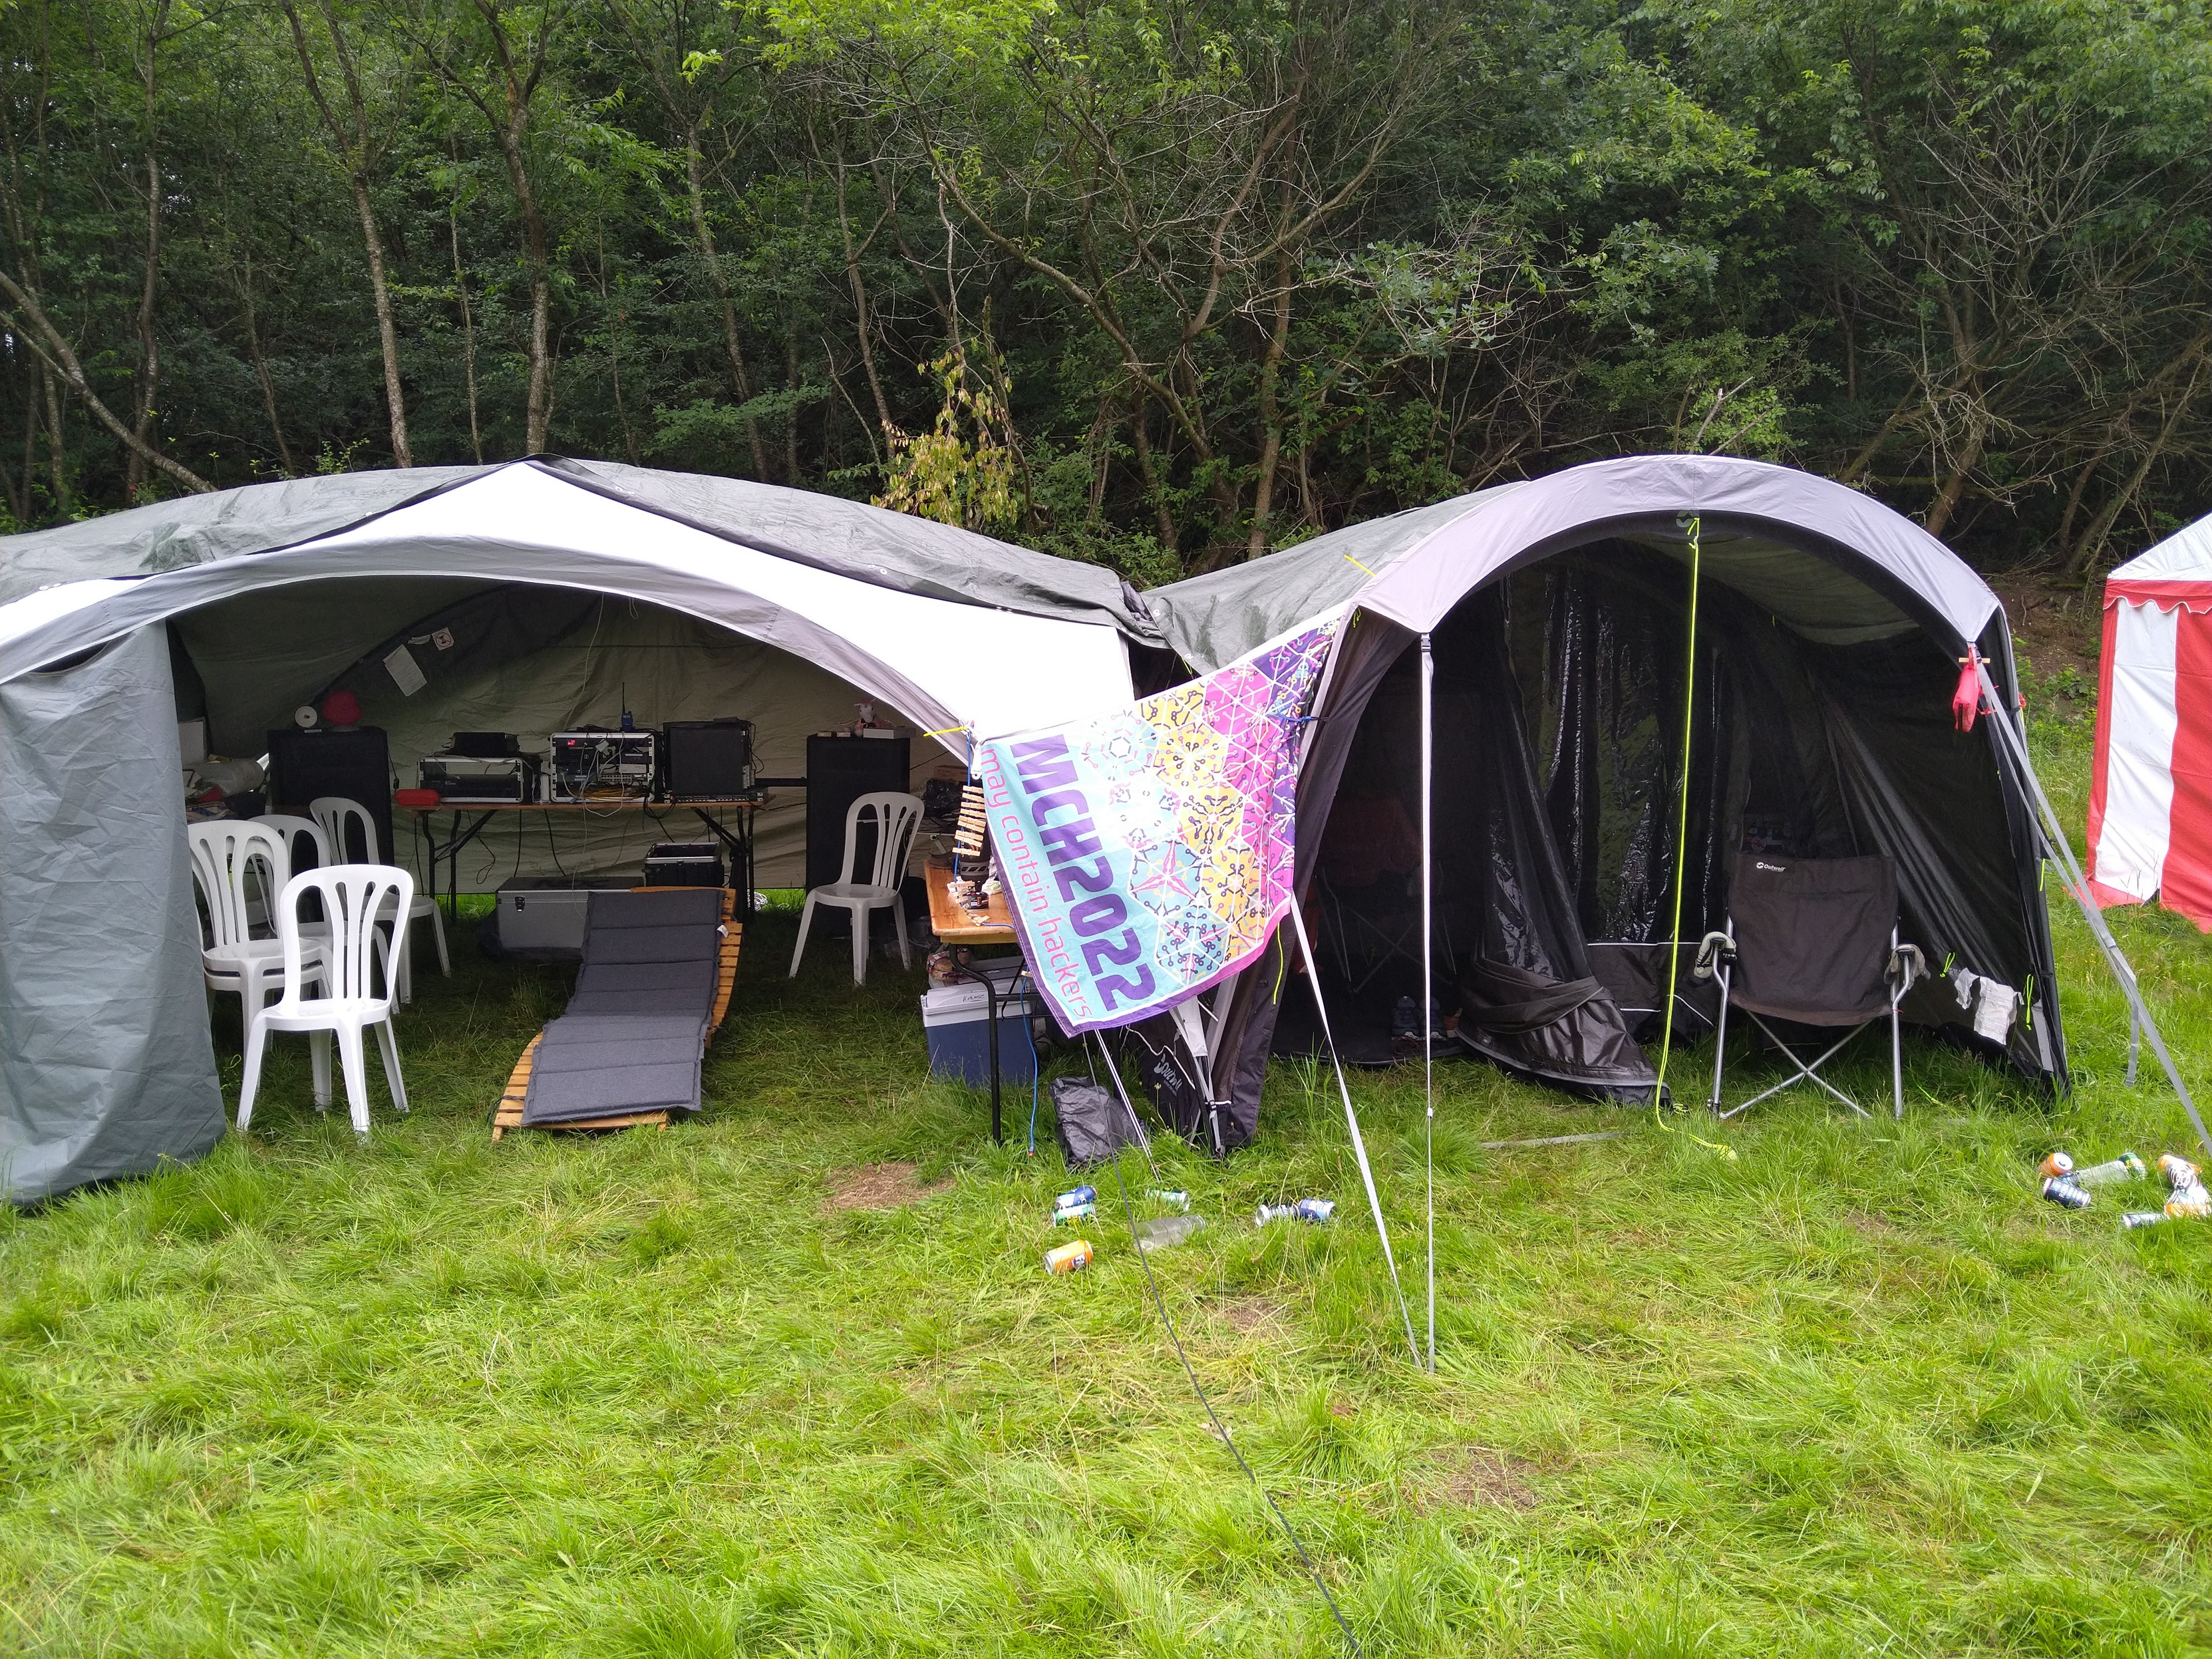
\includegraphics[width=10cm]{images/bornhack-camp-2024.jpg}}
\end{center}
\caption{The NWWC village at BornHack 2024, next year 16-23rd of July 2025}
\end{figure}


\eject

% =================== body of the document ===============
% Arabic page numbers
\pagenumbering{arabic}
\rhead{\fancyplain{}{\bf \chaptername\ \thechapter}}

% Main chapters
%---------------------------------------------------------------------
% gennemgang af emnet
% check questions


\chapter*{\color{titlecolor}Introduction to networking}
%\markboth{Introduktion til netværk}{}
\label{chap:intro}

\section*{\color{titlecolor}IP - Internet protocol suite}

It is extremely important to have a working knowledge about IP to implement
secure and robust infrastructures. Knowing about the alternatives while doing
implementation will allow the selection of the best features.

\section*{\color{titlecolor}ISO/OSI reference model}
A very famous model used for describing networking is the ISO/OSI model
of networking which describes layering of network protocols in stacks.

This model divides the problem of communicating into layers which can
then solve the problem as smaller individual problems and the solution
later combined to provide networking.

Having layering has proven also in real life to be helpful, for instance
replacing older hardware technologies with new and more efficient technologies
without changing the upper layers.

In the picture the OSI reference model is shown along side with
the Internet Protocol suite model which can also be considered to have different layers.


\begin{figure}[H]
\label{fig:osi}
\begin{center}
\colorbox{white}{\includegraphics[width=8cm,angle=90]{images/compare-osi-ip.pdf}}
\end{center}
\caption{OSI og Internet Protocol suite}
\end{figure}


\chapter*{\color{titlecolor}Exercise content}
\markboth{Exercise content}{}

Most exercises follow the same procedure and has the following content:
\begin{itemize}
\item {\bf Objective:} What is the exercise about, the objective
\item {\bf Purpose:} What is to be the expected outcome and goal of doing this exercise
\item {\bf Suggested method:} suggest a way to get started
\item {\bf Hints:} one or more hints and tips or even description how to
do the actual exercises
\item {\bf Solution:} one possible solution is specified
\item {\bf Discussion:} Further things to note about the exercises, things to remember and discuss
\end{itemize}

Please note that the method and contents are similar to real life scenarios and does not detail every step of doing the exercises. Entering commands directly from a book only teaches typing, while the exercises are designed to help you become able to learn and actually research solutions.



\chapter{\faInfoCircle\ Download Debian Administrator’s Handbook (DEB) Book 10 min}
\label{ex:sw-downloadDEB}

\hlkimage{3cm}{book-debian-administrators-handbook.jpg}


{\bf Objective:}\\
We need a Linux for running some tools during the course. I have chosen Debian Linux as this is open source, and the developers have released a whole book about running it.

This book is named
\emph{The Debian Administrator’s Handbook},  - shortened DEB

{\bf Purpose:}\\
Debian Linux is a mature Unix with great documentation. Kali Linux is based on Debian, so buy learning Debian you can make infrastructure using Debian Linux, and test security using Kali Linux -- and the administration will be the same commands.

in a few moments, so better have the instructions ready.

{\bf Suggested method:}\\
Create folders for educational materials. Go to download from the link \url{https://debian-handbook.info/}
Read and follow the instructions for downloading the book.

{\bf Solution:}\\
When you have a directory structure for download for this course, and the book DEB in PDF you are done.

{\bf Discussion:}\\
Linux is free and everywhere. The tools we will run in this course are made for Unix, so they run great on Linux.

Debian Linux is a free operating system platform.

The book DEB is free, but you can buy/donate to Debian, and I recommend it.


\chapter{\faInfoCircle\ Check your Debian VM 10 min}
\label{ex:sw-basicDebianVM}

\hlkimage{7cm}{debian-xfce.png}

{\bf Objective:}\\
I use Debian as the base for exercises -- they are tested on Debian and Kali!

If you want to use Debian, make sure your virtual machine is in working order.

You dont need both a Debian Linux and Kali for running tools in this booklet, but some are better suited for either, so you can choose to install both.

{\bf Purpose:}\\
If your VM is not installed and updated you might run into trouble later.

{\bf Suggested method:}\\
Go to \link{https://github.com/kramse/kramse-labs/}

Read the instructions for the setup of a Debian VM.

{\Large \bf This is a bonus exercise - only one Debian is needed per team.}

{\bf Hints:}\\
If you allocate enough memory and disk you wont have problems.

{\bf I suggest 50G disk, 2CPU cores and 6Gb memory for this course, if you have this.}

{\bf Solution:}\\
When you have a updated virtualisation software and a running VM, then we are good.

{\bf Discussion:}\\
Linux is free and everywhere. The tools we will run in this course are made for Unix, so they run great on Linux.

Debian Linux allows us to run Ansible and provision a whole SIEM in very few minutes.




\chapter{\faInfoCircle\ Configure Sudo}
\label{ex:configure-sudo}

{\bf Objective:}\\
Learn how to configure the tool Sudo to allow administrative commands.

{\bf Purpose:}\\
Sudo is the most common method for switching from a normal user to root which is the administrative user for Unix. This command allows you to use your own password and execute highly privileged commands easily.

{\bf Suggested method:}\\
Not in sudoers file, cannot run sudo command

This can be fixed quite easily.

If you use the su command first, to switch user to root and run the visudo command:
\begin{alltt}
hlk@debian01:~$ su -
// enter password
# visudo
\end{alltt}
You will get an editor, where you enter below the root line, your username and a similar line:
\begin{alltt}
# User privilege specification
root ALL = (ALL:ALL) ALL
hlk ALL = (ALL:ALL) NOPASSWD: ALL
\end{alltt}

In the example my user is \verb+hlk+

Then use ctrl-x if using Nano, and exit the editor - saving this configuration file.

{\bf Hints:}\\
Most books about Unix has a convention to use the dollar sign if you are logged in as a regular user and the hash tag sign when logged in as root.
\begin{alltt}
hlk@debian01:~$ echo "Hi I am just a regular user"

root@debian01:~# echo "this is a command being run by root"
\end{alltt}


{\bf Solution:}\\
When you can switch between your user and root you are done.

{\bf Discussion:}\\
Note sudo has had many security vulnerabilities, so you should keep your system up to date using apt regularly, read about updates in the DEB book.


\chapter{\faInfoCircle\ Enable firewall - 15min}
\label{ex:debian-firewall}

{\bf Objective:}\\
Turn on a firewall and configure a few simple rules.

{\bf Purpose:}\\
See how easy it is to restrict incoming connections to a server.


{\bf Suggested method:}\\
Install a utility for firewall configuration.

You should also perform Nmap port scan with the firewall enabled and disabled.

{\bf Hints:}\\
Using the ufw package it is very easy to configure the firewall on Linux.

Install and configuration can be done using these commands.
\begin{minted}[fontsize=\footnotesize]{shell}
root@debian01:~# apt install ufw
Reading package lists... Done
Building dependency tree
Reading state information... Done
The following NEW packages will be installed:
  ufw
0 upgraded, 1 newly installed, 0 to remove and 0 not upgraded.
Need to get 164 kB of archives.
After this operation, 848 kB of additional disk space will be used.
Get:1 http://mirrors.dotsrc.org/debian stretch/main amd64 ufw all 0.35-4 [164 kB]
Fetched 164 kB in 2s (60.2 kB/s)
...
root@debian01:~# ufw allow 22/tcp
Rules updated
Rules updated (v6)
root@debian01:~# ufw enable
Command may disrupt existing ssh connections. Proceed with operation (y|n)? y
Firewall is active and enabled on system startup
root@debian01:~# ufw status numbered
Status: active

     To                         Action      From
     --                         ------      ----
[ 1] 22/tcp                     ALLOW IN    Anywhere
[ 2] 22/tcp (v6)                ALLOW IN    Anywhere (v6)
\end{minted}

Also allow port 80/tcp and port 443/tcp - and install a web server. Recommend Nginx \verb+apt-get install nginx+

{\bf Solution:}\\
When firewall is enabled and you can still connect to Secure Shell (SSH) and web service, you are done.

{\bf Discussion:}\\
Further configuration would often require adding source prefixes which are allowed to connect to specific services. If this was a database server the database service should probably not be reachable from all of the Internet.

Web interfaces also exist, but are more suited for a centralized firewall.

Configuration of this firewall can be done using ansible, see the documentation and examples at \url{https://docs.ansible.com/ansible/latest/modules/ufw_module.html}

Should you have both a centralized firewall in front of servers, and local firewall on each server? Discuss within your team.



\chapter{\faInfoCircle\ Git tutorials - 15min}
\label{ex:git-tutorial}


\hlkimage{3cm}{git-logo.png}

{\bf Objective:}\\
Try the program Git locally on your workstation

{\bf Purpose:}\\
Running Git will allow you to clone repositories from others easily. This is a great way to get new software packages, and share your own.

Git is the name of the tool, and Github is a popular site for hosting git repositories.

{\bf Suggested method:}\\
Put Git on your list of technologies to learn.

If you feel like it, try the program from your Linux VM. You can also clone from your Windows or Mac OS X computer. Multiple graphical front-end programs exist too.

Most important are Git clone and pull:
\begin{alltt}\footnotesize
user@Projects:tt$ {\bf git clone https://github.com/kramse/kramse-labs.git}
Cloning into 'kramse-labs'...
remote: Enumerating objects: 283, done.
remote: Total 283 (delta 0), reused 0 (delta 0), pack-reused 283
Receiving objects: 100% (283/283), 215.04 KiB | 898.00 KiB/s, done.
Resolving deltas: 100% (145/145), done.

user@Projects:tt$ {\bf cd kramse-labs/}

user@Projects:kramse-labs$ {\bf ls}
LICENSE  README.md  core-net-lab  lab-network  suricatazeek  work-station
user@Projects:kramse-labs$ git pull
Already up to date.
\end{alltt}

{\bf Hints:}\\
Browse the Git tutorials on \link{https://git-scm.com/docs/gittutorial}\\
and \link{https://guides.github.com/activities/hello-world/}

We will not do the tutorials, but get an idea of the command line, and see examples. Refer back to these tutorials when needed or do them at home.

Note: you don't need an account on Github to download/clone repositories, but having an acccount allows you to save repositories yourself and is recommended.

{\bf Solution:}\\
When you have understood the importance of this tool and seen the tutorials you are done.

{\bf Discussion:}\\
Before Git there has been a range of version control systems,\\
see \link{https://en.wikipedia.org/wiki/Version\_control} for more details.




\hlkimage{6cm}{tcp-three-way.pdf}


{\bf Objective:}\\
Sniff TCP packets and dissect them using Wireshark

{\bf Purpose:}\\
See real network traffic, also know that a lot of information is available and not encrypted.

Note the three way handshake between hosts running TCP. You can either use a browser or command line tools like cURL while capturing

\begin{alltt}
curl http://www.zencurity.com
\end{alltt}

{\bf Suggested method:}\\
Open Wireshark and start a capture\\
Then in another window execute the ping program while sniffing

or perform a Telnet connection while capturing data

{\bf Hints:}\\
When running on Linux the network cards are usually named eth0 for the first Ethernet and wlan0 for the first Wireless network card. In Windows the names of the network cards are long and if you cannot see which cards to use then try them one by one.

{\bf Solution:}\\
When you have collected some TCP sessions you are done.

{\bf Discussion:}
Is it ethical to collect packets from an open wireless network?

Also note the TTL values in packets from different operating systems

\chapter{\faInfoCircle\ Whois databases 15 min}
\label{ex:whois}

{\bf Objective:}\\
Learn to lookup data in the global Whois databases

{\bf Purpose:}\\
We often need to see where traffic is coming from, or who is responsible for the IP addresses sending attacks.

{\bf Suggested method:}\\
Use a built-in command line, like: \verb+host www.zencurity.dk+ to look up an IP address and then \verb+whois + with the IP address.

{\bf Hints:}\\
Another option is to use web sites for doing Whois lookups \link{https://apps.db.ripe.net/db-web-ui/\#/query} or their RIPEStat web site which can give even more information
\link{https://stat.ripe.net/}

{\bf Solution:}\\
When you can find our external address and look it up, you are done.

{\bf Discussion:}\\
Whois databases are global and used for multiple purposes, the ones run by the Regional Internet Registries ARIN, RIPE, AfriNIC, LACNIC og APNIC have information about IP addresses and AS numbers allocated.


\chapter{\faInfoCircle\ IP address research 30 min}
\label{ex:ip-address-research}

{\bf Objective:}\\
Work with IP addresses

{\bf Purpose:}\\
What is an IP address?

Investigate the following IP addresses
\begin{list2}
\item 192.168.1.1
\item 192.0.2.0/24
\item 172.25.0.1
\item 182.129.62.63
\item 185.129.62.63
\end{list2}

Write down everything you can about them!

{\bf Suggested method:}\\
Search for the addresses, look for web sites that may help.

{\bf Hints:}\\
Download the fun guide from Julia Evans (b0rk) \url{https://jvns.ca/networking-zine.pdf}

Pay attention to Notation Time page

Lookup \url{ripe.net} they may have a service called stats or stat -- something like that.

What is the Torproject? good, bad, neutral?

{\bf Solution:}\\
When you have found some information about each of the above, say 2-3 facts about each you are done.

{\bf Discussion:}\\
IP addresses are much more than an integer used for addressing system interfaces and routing packets.

We will later talk more about \emph{IP reputation}


\chapter{\faInfoCircle\ Using ping and traceroute 10 min}
\label{ex:ping}



{\bf Objective:}\\
Be able to do initial debugging of network problems using commands ping and traceroute

{\bf Purpose:}\\
Being able to verify connectivity is a basic skill.

{\bf Suggested method:}\\
Use \verb+ping+ and \verb+traceroute+ to test your network connection - can be done one Windows and UNIX.

{\bf Hints:}
\begin{alltt}\small
$ ping 10.0.42.1
PING 10.0.42.1 (10.0.42.1) 56(84) bytes of data.
64 bytes from 10.0.42.1: icmp_seq=1 ttl=62 time=1.02 ms
64 bytes from 10.0.42.1: icmp_seq=2 ttl=62 time=0.998 ms
^C
--- 10.0.42.1 ping statistics ---
2 packets transmitted, 2 received, 0% packet loss, time 1001ms
rtt min/avg/max/mdev = 0.998/1.012/1.027/0.034 ms
\end{alltt}

Dont forget that UNIX ping continues by default, press ctrl-c to break.

Do the same with traceroute.

{\bf Solution:}\\
Run both programs to local gateway and some internet address by your own choice.

{\bf Discussion:}\\
Note the tool is called tracert on Windows, shortened for some reason.

ICMP is the Internet Control Message Protocol, usually used for errors like host unreachable. The ECHO request ICMP message is the only ICMP message that generates another.

The traceroute programs send packets with low Time To Live (TTL) and receives ICMP messages, unless there is a problem or a firewall/filter. Also used for mapping networks.

{\bf \faInfoCircle\ }

Whats the difference between:
\begin{list2}
\item {\bfseries traceroute} and {\bfseries traceroute -I}
\item NB: traceroute -I is found on UNIX - traceroute using ICMP pakker
\item Windows tracert by default uses ICMP
\item Unix by default uses UDP, but can use ICMP instead.
\item Lots of traceroute-like programs exist for tracing with TCP or other protocols
\end{list2}


\chapter{\faInfoCircle\ DNS and Name Lookups 10 min}
\label{ex:basic-dns-lookup}



{\bf Objective:}\\
Be able to do DNS lookups from specific DNS server

{\bf Purpose:}\\
Try doing DNS lookup using different programs

{\bf Suggested method:}\\
Try the following programs:
\begin{itemize}
\item nslookup - UNIX and Windows, but not recommended\\
\verb+nslookup -q=txt -class=CHAOS version.bind. 0+
\item dig - syntax @server domain query-type query-class\\
\verb+dig @8.8.8.8 www.example.com+
\item host - syntaks host [-l] [-v] [-w] [-r] [-d] [-t querytype] [-a] host [server]\\
\verb+host www.example.com 8.8.8.8+
\end{itemize}

{\bf Hints:}\\
Dig is the one used by most DNS admins, I often prefer the host command for the short output.

{\bf Solution:}\\
Shown inline, above.

{\bf Discussion:}\\
The nslookup program does not use the same method for lookup as the standard lookup libraries, results may differ from what applications see.

What is a zone transfer, can you get one using the host command?

Explain forward and reverse DNS lookup.




\chapter{\faInfoCircle\ Nping check ports 10 min}
\label{ex:nping-tcp}
{\bf Objective:} \\
Show the use of Nping tool for checking ports through a network

{\bf Purpose:}\\
Nping can check if probes can reach through a network, reporting success of failure. Allows very specific packets to be sent. It is part of the Nmap package.

{\bf Suggested method:}\\
Run the command using a common port like Web HTTP:
\begin{alltt}\footnotesize
root@KaliVM:~# nping --tcp -p 80 www.zencurity.com

Starting Nping 0.7.70 ( https://nmap.org/nping ) at 2018-09-07 19:06 CEST
SENT (0.0300s) TCP 10.137.0.24:3805 > 185.129.60.130:80 S ttl=64 id=18933 iplen=40  seq=2984847972 win=1480
RCVD (0.0353s) TCP 185.129.60.130:80 > 10.137.0.24:3805 SA ttl=56 id=49674 iplen=44  seq=3654597698 win=16384 <mss 1460>
SENT (1.0305s) TCP 10.137.0.24:3805 > 185.129.60.130:80 S ttl=64 id=18933 iplen=40  seq=2984847972 win=1480
RCVD (1.0391s) TCP 185.129.60.130:80 > 10.137.0.24:3805 SA ttl=56 id=50237 iplen=44  seq=2347926491 win=16384 <mss 1460>
SENT (2.0325s) TCP 10.137.0.24:3805 > 185.129.60.130:80 S ttl=64 id=18933 iplen=40  seq=2984847972 win=1480
RCVD (2.0724s) TCP 185.129.60.130:80 > 10.137.0.24:3805 SA ttl=56 id=9842 iplen=44  seq=2355974413 win=16384 <mss 1460>
SENT (3.0340s) TCP 10.137.0.24:3805 > 185.129.60.130:80 S ttl=64 id=18933 iplen=40  seq=2984847972 win=1480
RCVD (3.0387s) TCP 185.129.60.130:80 > 10.137.0.24:3805 SA ttl=56 id=1836 iplen=44  seq=3230085295 win=16384 <mss 1460>
SENT (4.0362s) TCP 10.137.0.24:3805 > 185.129.60.130:80 S ttl=64 id=18933 iplen=40  seq=2984847972 win=1480
RCVD (4.0549s) TCP 185.129.60.130:80 > 10.137.0.24:3805 SA ttl=56 id=62226 iplen=44  seq=3033492220 win=16384 <mss 1460>

Max rtt: 40.044ms | Min rtt: 4.677ms | Avg rtt: 15.398ms
Raw packets sent: 5 (200B) | Rcvd: 5 (220B) | Lost: 0 (0.00%)
Nping done: 1 IP address pinged in 4.07 seconds
\end{alltt}

{\bf Hints:} \\
A lot of options are similar to Nmap

{\bf Solution:}\\
When you have tried it towards an open port, a closed port and an IP/port that is filtered you are done.

{\bf Discussion:}\\
A colleague of ours had problems sending specific IPsec packets through a provider. Using a tool like Nping it is possible to show what happens, or where things are blocked.

\eject
Things like changing the TTL may provoke ICMP messages, like this:
\begin{alltt}\footnotesize
root@KaliVM:~# nping --tcp -p 80 --ttl 3 www.zencurity.com

Starting Nping 0.7.70 ( https://nmap.org/nping ) at 2018-09-07 19:08 CEST
SENT (0.0303s) TCP 10.137.0.24:37244 > 185.129.60.130:80 S ttl=3 id=60780 iplen=40  seq=1997801125 win=1480
RCVD (0.0331s) ICMP [10.50.43.225 > 10.137.0.24 TTL=0 during transit (type=11/code=0) ] IP [ttl=62 id=28456 iplen=72 ]
SENT (1.0314s) TCP 10.137.0.24:37244 > 185.129.60.130:80 S ttl=3 id=60780 iplen=40  seq=1997801125 win=1480
RCVD (1.0337s) ICMP [10.50.43.225 > 10.137.0.24 TTL=0 during transit (type=11/code=0) ] IP [ttl=62 id=28550 iplen=72 ]
SENT (2.0330s) TCP 10.137.0.24:37244 > 185.129.60.130:80 S ttl=3 id=60780 iplen=40  seq=1997801125 win=1480
RCVD (2.0364s) ICMP [10.50.43.225 > 10.137.0.24 TTL=0 during transit (type=11/code=0) ] IP [ttl=62 id=28589 iplen=72 ]
SENT (3.0346s) TCP 10.137.0.24:37244 > 185.129.60.130:80 S ttl=3 id=60780 iplen=40  seq=1997801125 win=1480
RCVD (3.0733s) ICMP [10.50.43.225 > 10.137.0.24 TTL=0 during transit (type=11/code=0) ] IP [ttl=62 id=29403 iplen=72 ]
SENT (4.0366s) TCP 10.137.0.24:37244 > 185.129.60.130:80 S ttl=3 id=60780 iplen=40  seq=1997801125 win=1480
RCVD (4.0558s) ICMP [10.50.43.225 > 10.137.0.24 TTL=0 during transit (type=11/code=0) ] IP [ttl=62 id=30235 iplen=72 ]

Max rtt: 38.574ms | Min rtt: 2.248ms | Avg rtt: 13.143ms
Raw packets sent: 5 (200B) | Rcvd: 5 (360B) | Lost: 0 (0.00%)
Nping done: 1 IP address pinged in 4.07 seconds
\end{alltt}



\chapter{\faInfoCircle\ Wireshark and Tcpdump 15 min}
\label{ex:wireshark-install}

\hlkimage{10cm}{wireshark-http.png}


{\bf Objective:}\\
Try the program Wireshark locally your workstation, or tcpdump

You can run Wireshark on your host too, if you want.

{\bf Purpose:}\\
Installing Wireshark will allow you to analyse packets and protocols

Tcpdump is a feature included in many operating systems and devices to allow packet capture and saving network traffic into files.

{\bf Suggested method:}\\
Run Wireshark or tcpdump 

The PPA book page 41 describes Your First Packet Capture.

{\bf Hints:}\\
PCAP is a packet capture library allowing you to read packets from the network.
Tcpdump uses libpcap library to read packet from the network cards and save them.
Wireshark is a graphical application to allow you to browse through traffic, packets and protocols.

Both tools are already on your Kali Linux, or do: \verb+apt-get install tcpdump wireshark+

{\bf Solution:}\\
When Wireshark is installed sniff some packets. We will be working with both live traffic and saved packets from files in this course.

If you want to capture packets as a non-root user on Debian, then use the command to add a Wireshark group:
\begin{alltt}
sudo dpkg-reconfigure wireshark-common
\end{alltt}

and add your user to this:
\begin{alltt}
sudo gpasswd -a $USER wireshark
\end{alltt}
Dont forget to logout/login to pick up this new group.

{\bf Discussion:}\\
Wireshark is just an example other packet analyzers exist, some commercial and some open source like Wireshark

We can download a lot of packet traces from around the internet, we might use examples from\\
\link{https://old.zeek.org/community/traces.html}


\chapter{\faInfoCircle\ Discover active systems ping sweep 10 min}
\label{ex:nmap-pingsweep}
\hlkimage{5cm}{nmap-zenmap.png}

{\bf Objective:}\\
Use nmap to discover active systems

{\bf Purpose:}\\
Know how to use nmap to scan networks for active systems.

{\bf Suggested method:}\\
Try different scans,
\begin{itemize}
\item Ping sweep to find active systems
\item Port sweeps to find active systems with specific ports
\end{itemize}

{\bf Hints:} \\
Try nmap in sweep mode - and you may run this from Zenmap

{\bf Solution:}\\
Use the command below as examples:
\begin{itemize}
\item Ping sweep \verb+nmap -sP 10.0.45.*+
\item Port sweeps \verb+nmap -p 80 10.0.45.*+
\end{itemize}

{\bf Discussion:}\\
Quick scans quickly reveal interesting hosts, ports and services

Also now make sure you understand difference between single host scan
10.0.45.123/32, a whole subnet /24 ~250 hosts 10.0.45.0/24 and other more advanced targeteting like 10.0.45.0/25 and 10.0.45.1-10


\chapter{\faInfoCircle\ Execute nmap TCP and UDP port scan 20 min}
\label{ex:nmap-synscan}


{\bf Objective:} \\
Use nmap to discover important open ports on active systems

{\bf Purpose:}\\
Finding open ports will allow you to find vulnerabilities on these ports.

{\bf Suggested method:}\\
Use \verb+nmap -p 1-1024 server+ to scan the first 1024 TCP
ports and use Nmap without ports. What is scanned then?

Try to use \verb+nmap -sU+ to scan using UDP ports, not really possible if a firewall is in place.

If a firewall blocks ICMP you might need to add \verb+-Pn+ to make nmap scan even if there are no Ping responses

{\bf Hints:} \\
Sample command: \verb+nmap -Pn -sU -p1-1024 server+ UDP port scanning
1024 ports without doing a Ping first

{\bf Solution:}\\
Discover some active systems and most interesting ports, which are 1-1024 and the built-in list of popular ports.

{\bf Discussion:}\\
There is a lot of documentation about the nmap portscanner, even a book by the author
of nmap. Make sure to visit \link{http://www.nmap.org}

TCP and UDP is very different when scanning. TCP is connection/flow oriented and requires a handshake which is very easy to identify. UDP does not have a handshake and most applications will not respond to probes from nmap. If there is no firewall the operating system will respond to UDP probes on closed ports - and the ones that do not respond must be open.

When doing UDP scan on the internet you will almost never get a response, so you cannot tell open (not responding services) from blocked ports (firewall drop packets). Instead try using specific service programs for the services, sample program could be \verb+nsping+ which sends DNS packets, and will often get a response from a DNS server running on UDP port 53.

\chapter{\faInfoCircle\ Perform nmap OS detection 10 min}
\label{ex:nmap-os}

{\bf Objective:} \\
Use nmap OS detection and see if you can guess the brand of devices on the network

{\bf Purpose:}\\
Getting the operating system of a system will allow you to focus your next attacks.

{\bf Suggested method:}\\
Look at the list of active systems, or do a ping sweep.

Then add the OS detection using the option \verb+-O+ -- or \verb+-A+ which also add even more good stuff.



{\bf Hints:} \\
The nmap tool can send a lot of packets that will get different responses, depending on the operating system. TCP/IP is implemented using various constants chosen by the implementors, they have chosen different standard packet TTL etc.

{\bf Solution:}\\
Use a command like \verb+nmap -O -p1-100 10.0.45.45+ or  \verb+nmap -A -p1-100 10.0.45.45+


{\bf Discussion:}\\
Nmap OS detection is not a full proof way of knowing the actual operating system, but in most cases in can detect the family and in some cases it can identify the exact patch level of the system.

Better to use \verb+-A+ all the time, includes even more scripts and advanced stuff
You can also save prefixes to scan in a text file, I usually name it \verb+targets+

I also recommend adding \verb+-oA+ for writing output files. So a regular Nmap command might be:
\verb+nmap -p 1-65535 -A -oA full-tcp-scan -iL targets+



\chapter{\faInfoCircle\ TCP SYN flooding 30min}
\label{ex:syn-flood}

{\bf Objective:}\\
Start a webserver attack using SYN flooding tool hping3.

{\bf Purpose:}\\
See how easy it is to produce packets on a network using hacker programs.

The tool we will use is very flexible and can produce ICMP, UDP and TCP using very few options. This tool is my primary one for doing professsional DDoS testing.

\begin{alltt}\footnotesize
-1 --icmp
       ICMP  mode,  by  default  hping3  will  send  ICMP echo-request, you can set other ICMP
       type/code using --icmptype --icmpcode options.

-2 --udp
       UDP mode, by default hping3 will send udp to target host's port 0.  UDP header  tunable
       options are the following: --baseport, --destport, --keep.
\end{alltt}

TCP mode is default, so no option needed.


{\bf Suggested method:}\\
Connect to the LAB network using Ethernet! Borrow a USB network card if you dont have one.

Start your Kali VM in bridged mode, try a basic TCP flooding attack against the server provided by the instructor, or your own Debian server.

Try doing the most common attacks TCP SYN flood using hping3:

\begin{alltt}
hping3 --flood -p 80 -S 10.0.45.12
\end{alltt}

You should see something like this:
\begin{alltt}\footnotesize
HPING 10.0.45.12: NO FLAGS are set, 40 headers + 0 data bytes
hping in flood mode, no replies will be shown
^C
--- 10.0.45.12 hping statistic ---
352339 packets transmitted, 0 packets received, 100% packet loss
round-trip min/avg/max = 0.0/0.0/0.0 ms
\end{alltt}

You can try different ports with TCP flooding, try port 22/tcp or HTTP(S) port 80/tcp and 443/tcp


{\bf Hints:}\\
The tool we use can do a lot of different things, and you can control the speed. You can measure at the server being attacked or what you are sending, commonly using ifpps or such programs can help.

By changing the speed we can find out how much traffic is needed to bring down a service. This measurement can then be re-checked later and see if improvements really worked.

This allows you to use the tool to test devices and find the breaking point, which is more interesting than if you can overload, because you always can.
\begin{alltt}\footnotesize
-i --interval
       Wait  the  specified  number  of  seconds or micro seconds between sending each packet.
       --interval X set wait to X seconds, --interval uX set wait to X micro seconds.  The de‐
       fault  is  to  wait one second between each packet. Using hping3 to transfer files tune
       this option is really important in order to increase transfer rate. Even  using  hping3
       to  perform  idle/spoofing  scanning  you should tune this option, see HPING3-HOWTO for
       more information.

--fast Alias for -i u10000. Hping will send 10 packets for second.

--faster
       Alias for -i u1. Faster then --fast ;) (but not as fast as your computer can send pack‐
       ets due to the signal-driven design).

--flood
       Sent  packets  as fast as possible, without taking care to show incoming replies.  This
       is ways faster than to specify the -i u0 option.
\end{alltt}

{\bf Solution:}\\
When your team has sent +1 million packets per second into the network, from one or two laptops - you are done.

{\bf Discussion:}\\
Gigabit Ethernet can send up to 1.4 million packets per second, pps.

There is a presentation about DDoS protection with low level technical measures to implement at\\
{\footnotesize \link{https://github.com/kramse/security-courses/tree/master/presentations/network/introduction-ddos-testing}}

Receiving systems, and those en route to the service, should be checked for resources like CPU load, bandwidth, logging. Logging can also overload the logging infrastructure, so take care when configuring this in your own networks.


\chapter{\faInfoCircle\ TCP other flooding 15min}


{\bf Objective:}\\
Start a webserver attack using TCP flooding tool hping3.

{\bf Purpose:}\\
Run various other common attacks

TCP mode is default, so no option needed.


{\bf Suggested method:}\\
Connect to the LAB network using Ethernet! Borrow a USB network card if you dont have one.

Start your Kali VM in bridged mode, try a basic TCP flooding attack against the server provided by the instructor, or your own Debian server.

\begin{alltt}
hping3 --flood -p 80 -R 10.0.45.12
\end{alltt}

You should see something like this:
\begin{alltt}\footnotesize
HPING 10.0.45.12: NO FLAGS are set, 40 headers + 0 data bytes
hping in flood mode, no replies will be shown
^C
--- 10.0.45.12 hping statistic ---
352339 packets transmitted, 0 packets received, 100% packet loss
round-trip min/avg/max = 0.0/0.0/0.0 ms
\end{alltt}


{\bf Hints:}\\
Common attacks use the SYN, as shown in previous exercise, but other popular
TCP attacks are RST, PUSH, URG, FIN, ACK attacks - setting one or more flags in the packets.

\begin{alltt}
-L  --setack     set TCP ack
-F  --fin        set FIN flag
-S  --syn        set SYN flag
-R  --rst        set RST flag
-P  --push       set PUSH flag
-A  --ack        set ACK flag
-U  --urg        set URG flag
-X  --xmas       set X unused flag (0x40)
-Y  --ymas       set Y unused flag (0x80)
\end{alltt}





{\bf Solution:}\\
When your team has sent +1 million packets per second into the network, from one or two laptops - you are done.

{\bf Discussion:}\\
If an attacker varies the packets they can be harder to filter out, and the attacks succeed.

\chapter{\faInfoCircle\ UDP flooding NTP, etc. 15min}


{\bf Objective:}\\
Start a webserver attack using UDP flooding tool hping3.

{\bf Purpose:}\\
See how easy it is to produce packets on a network using hacker programs.

The tool we will use is very flexible and can produce ICMP, UDP and TCP using very few options. This tool is my primary one for doing professsional DDoS testing.

This time we will select UDP mode:

\begin{alltt}\footnotesize
-2 --udp
       UDP mode, by default hping3 will send udp to target host's port 0.  UDP header  tunable
       options are the following: --baseport, --destport, --keep.
\end{alltt}

{\bf Suggested method:}\\
Connect to the LAB network using Ethernet! Borrow a USB network card if you dont have one.

Start your Kali VM in bridged mode, try a basic TCP flooding attack against the server provided by the instructor, or your own Debian server.

\begin{alltt}\footnotesize
hping3 --flood -2 -p 53 10.0.45.12
\end{alltt}



{\bf Hints:}\\

Try doing the most common attacks:
\begin{itemize}
\item UDP flooding, try port 53/udp DNS, 123/udp NTP and port 161/udp SNMP
\end{itemize}

{\bf Solution:}\\
When your team has sent +1 million packets per second into the network, from one or two laptops - you are done.

{\bf Discussion:}\\
Many networks don't send and receive a lot of UDP traffic. If you measure a baseline of the protocols needed on a daily basis you might be able to configure a profile for normal usage, and filter out bad traffic in case of attacks.

A starting point might be to allow full bandwidth for TCP, 10\% UDP and 1\% ICMP. This will ensure that even if an attacker is sending more than 1\% ICMP only a fraction reaches your network and systems.

This is especially effective for protocols like ICMP which is not used for large data transfers.

\chapter{\faInfoCircle\ ICMP flooding 15min}

{\bf Objective:}\\
Start a webserver attack using ICMP flooding tool hping3.

{\bf Purpose:}\\
See how easy it is to produce packets on a network using hacker programs.

The tool we will use is very flexible and can produce ICMP, UDP and TCP using very few options. This tool is my primary one for doing professsional DDoS testing.

This time we will select UDP mode:

\begin{alltt}\footnotesize
-1 --icmp
       ICMP  mode,  by  default  hping3  will  send  ICMP echo-request, you can set other ICMP
       type/code using --icmptype --icmpcode options.
\end{alltt}

{\bf Suggested method:}\\
Connect to the LAB network using Ethernet! Borrow a USB network card if you dont have one.

Start your Kali VM in bridged mode, try a basic TCP flooding attack against the server provided by the instructor, or your own Debian server.

Try doing the most common attack:
\begin{itemize}
\item ICMP flooding with echo
\end{itemize}

\begin{alltt}\footnotesize
hping3 --flood -1 10.0.45.12
\end{alltt}





{\bf Hints:}\\
Common attacks use ICMP ECHO, but other types can be sent in the packets.

\begin{alltt}\footnotesize
ICMP
  -C  --icmptype   icmp type (default echo request)
  -K  --icmpcode   icmp code (default 0)
      --force-icmp send all icmp types (default send only supported types)
      --icmp-gw    set gateway address for ICMP redirect (default 0.0.0.0)
      --icmp-ts    Alias for --icmp --icmptype 13 (ICMP timestamp)
      --icmp-addr  Alias for --icmp --icmptype 17 (ICMP address subnet mask)
      --icmp-help  display help for others icmp options
\end{alltt}


{\bf Solution:}\\
When your team has sent +1 million packets per second into the network, from one or two laptops - you are done.

{\bf Discussion:}\\
If you have a 10G network connection, do you REALLY need 10Gbps of ICMP traffic?

Probably not, and routers can often filter this in wirespeed.

Routers have extensive Class-of-Service (CoS) tools today and a starting point might be as shown in Juniper Junos policer config:

\begin{alltt}\footnotesize
term limit-icmp \{
    from \{
        protocol icmp;
    \}
    then \{
        policer ICMP-100M;
        accept;
    \}
\}
term limit-udp \{
    from \{
        protocol udp;
    \}
    then \{
        policer UDP-1000M;
        accept;
    \}
\}
\end{alltt}

This effectively limit the damage an attacker can do. Your firewall and IDS devices will be free to spend more processing on the remaining protocols.



\chapter{\faInfoCircle\ Misc - stranger attacks 15min}

Various other attacks are possible, sending illegal combinations of flags etc.



{\bf Objective:}\\
Start a webserver attack using the packet generator and flooding tool t50.

{\bf Purpose:}\\
See how easy it is to produce packets on a network using hacker programs.

The tool we will use is very flexible and can produce ICMP, UDP and TCP using very few options. This tool is another primary one for doing professsional DDoS testing.

Apart from TCP,UDP and ICMP this tool can also produce packets for dynamic routing testting, OSPF, EIGRP and other esoteric RSVP, IPSEC, RIP and GRE.

\begin{alltt}\footnotesize
  $ t50 -help
  T50 Experimental Mixed Packet Injector Tool v5.8.3
  Originally created by Nelson Brito <nbrito@sekure.org>
  Previously maintained by Fernando Mercês <fernando@mentebinaria.com.br>
  Maintained by Frederico Lamberti Pissarra <fredericopissarra@gmail.com>

  Usage: t50 <host[/cidr]> [options]
  Common Options:
      --threshold NUM           Threshold of packets to send     (default 1000)
      --flood                   This option supersedes the 'threshold'
      --encapsulated            Encapsulated protocol (GRE)      (default OFF)
   -B,--bogus-csum              Bogus checksum                   (default OFF)
      --shuffle                 Shuffling for T50 protocol       (default OFF)
   -q,--quiet                   Disable INFOs
      --turbo                   Extend the performance           (default OFF)
   -l,--list-protocols          List all available protocols
   -v,--version                 Print version and exit
   -h,--help                    Display this help and exit
...
   Some considerations while running this program:
    1. There is no limitation of using as many options as possible.
    2. Report t50 bugs at https://gitlab.com/fredericopissarra/t50.git.
    3. Some header fields with default values MUST be set to '0' for RANDOM.
    4. Mandatory arguments to long options are mandatory for short options too.
    5. Be nice when using t50, the author DENIES its use for DoS/DDoS purposes.
    6. Running t50 with '--protocol T50' option sends ALL protocols sequentially.

\end{alltt}


{\bf Suggested method:}\\
Connect to the LAB network using Ethernet! Borrow a USB network card if you dont have one.

Start your Kali VM in bridged mode, try a basic TCP flooding attack against the server provided by the instructor, or your own Debian server.

Run the help page, and browse options.
\begin{alltt}\footnotesize
t50 -h
\end{alltt}





{\bf Hints:}\\
The tools we use can do a lot of different things and using the command line options can produce high speed packet attacks without having to program in C ourselves.

Try doing a special attack:
\begin{itemize}
\item t50 with '--protocol T50' option sends ALL protocols, so try:\\
\verb+t50 --protocol T50 10.0.45.12+
\end{itemize}


{\bf Solution:}\\
When your team has sent +1 million packets per second into the network, from one or two laptops - you are done.

{\bf Discussion:}\\
Gigabit Ethernet can send up to 1.4 million packets per second, pps.

There is a presentation about DDoS protection with low level technical measures to implement at\\
{\footnotesize \link{https://github.com/kramse/security-courses/tree/master/presentations/network/introduction-ddos-testing}}

Receiving systems, and those en route to the service, should be checked for resources like CPU load, bandwidth, logging. Logging can also overload the logging infrastructure, so take care when configuring this in your own networks.





\chapter{\faInfoCircle\ SSL/TLS scanners 15 min}
\label{ex:SSLScanner}

{\bf Objective:}\\
Try the Online Qualys SSLLabs scanner \link{https://www.ssllabs.com/}
Try the command line tool sslscan checking servers - can check both HTTPS and non-HTTPS protocols!

{\bf Purpose:}\\
Learn how to efficiently check TLS settings on remote services.

{\bf Suggested method:}\\
Run the tool against a couple of sites of your choice.

\begin{alltt}\small
root@kali:~# sslscan --ssl2 www.kramse.dk
Version: 1.10.5-static
OpenSSL 1.0.2e-dev xx XXX xxxx

Testing SSL server www.kramse.dk on port 443
...
  SSL Certificate:
Signature Algorithm: sha256WithRSAEncryption
RSA Key Strength:    2048

Subject:  *.kramse.dk
Altnames: DNS:*.kramse.dk, DNS:kramse.dk
Issuer:   AlphaSSL CA - SHA256 - G2
\end{alltt}

Also run it without \verb+--ssl2+ and against SMTPTLS if possible.

{\bf Hints:}\\
Originally sslscan is from \link{http://www.titania.co.uk} but use the version on Kali, install with apt if not installed.

{\bf Solution:}\\
When you can run and understand what the tool does, you are done.

{\bf Discussion:}\\
SSLscan can check your own sites, while Qualys SSLLabs only can test from hostname


\chapter{\faInfoCircle\ Internet scanners 15 min}
\label{ex:web-site-check}

{\bf Objective:}\\
Try the Online scanners \link{https://internet.nl/} and a few more.

{\bf Purpose:}\\
Learn how to efficiently check settings on remote services.

{\bf Suggested method:}\\
There are multiple portals and testing services which allow you to checck a domain,
mail settings or web site.

Run tools against a couple of sites of your choice.
\begin{itemize}
\item \url{https://internet.nl/} Generic checker
\item \url{https://www.hardenize.com/} Generic checker
\item \url{https://www.wormly.com/test_ssl} Test TLS
\item \url{https://observatory.mozilla.org/} Web site headers check
\item \url{https://dnsviz.net/} DNS zone check
\item \url{https://rpki.cloudflare.com/} Check RPKI - route validator enter
IP address\\
More information about this: \url{https://labs.ripe.net/author/nathalie_nathalie/rpki-test/}
\end{itemize}

Others exist, feel free to suggest some.

{\bf Hints:}\\

{\bf Solution:}\\
When you can run and understand what at least one tool does, you are done.

{\bf Discussion:}\\
Which settings are most important, which settings are your responsebility?


\chapter{\faInfoCircle\ Wireguard - 60 min}
\label{ex:wireguard-setup}

{\bf Objective:}\\
Research the \emph{new} wireguard between two Linux servers


{\bf Purpose:}\\
Know there is alternative to connect servers securely.

Wireguard is very easy to setup, as it requires very little configuration.


{\bf Suggested method:}\\
Find devices and operating systems that support Wireguard

Linux and OpenBSD can do it out-of-the-box
\link{https://www.wireguard.com/quickstart/}


{\bf Hints:}\\
They have a Demo Server which allows you to try out Wireguard

{\bf Solution:}\\
When you have a working connection between them, you are done.

{\bf Discussion:}\\
We wont do this in class, but I have a lot of friends that use Wireguard in production for complex setups.





\chapter{\faInfoCircle\ Zeek on the web 10min}
\label{ex:zeekweb}


{\bf Objective:} \\
Try Zeek Network Security Monitor - without installing it.


{\bf Purpose:}\\
Show a couple of examples of Zeek scripting, the built-in language found in Zeek Network Security Monitor


{\bf Suggested method:}\\
Go to \url{http://try.zeek.org/#/?example=hello} and try a few of the examples.

{\bf Hints:}\\
The exercise
\emph{The Summary Statistics Framework} can be run with a specifc PCAP.

\verb+192.168.1.201 did 402 total and 2 unique DNS requests in the last 6 hours.+

{\bf Solution:}\\
You should read the example \emph{Raising a Notice}. Getting output for certain events may be interesting to you.


{\bf Discussion:}\\
Zeek Network Security Monitor is an old/mature tool, but can still be hard to get started using. I would suggest that you always start out using the packages available in your Ubuntu/Debian package repositories.  They work, and will give a first impression of Zeek. If you later want specific features not configured into the binary packages, then install from source.

The tool was renamed in 2018 from Bro to Zeek. Some commands and files still reference the old names.

Also Zeek uses a zeekctl program to start/stop the tool, and a few config files which we should look at. From a Debian system they can be found in \verb+/opt/zeek/etc+ :

This is from the Debian 11 package, checked May 2022

\verb+/opt/zeek/etc+:
\begin{alltt}
root@debian-lab-11:/opt/zeek/etc# ls -la
total 24
drwxrwsr-x  3 root zeek 4096 Apr 16 20:03 .
drwxr-xr-x 10 root root 4096 Apr 16 20:03 ..
-rw-rw-r--  1 root zeek  262 Jan 28  2015 networks.cfg
-rw-rw-r--  1 root zeek  651 Jan 28  2015 node.cfg
-rw-rw-r--  1 root zeek 3052 Jan 28  2015 zeekctl.cfg
drwxr-xr-x  2 root zeek 4096 Apr 16 20:03 zkg
\end{alltt}




\chapter{\faInfoCircle\ Test a DNS server 30min}
\label{ex:dns-server-test}

{\bf Objective:}\\
Try communicating with DNS commands.

{\bf Purpose:}\\
Learn how basic the setup of Unbound DNS server is.

{\bf Suggested method:}\\
Setup Unbound on Debian using the instructions from\\
\link{https://nlnetlabs.nl/documentation/unbound/howto-setup/}

Note: there is a binary unbound package which can be installed with \verb+apt install unbound+ so use that, and config is then in \verb+/etc/unbound+ .

Use command line tools to test your server, if not available try ping - which will do a lookup. Retry the commands from exercise: {\bf \nameref{ex:basic-dns-lookup}}
which is number {\bf \ref{ex:basic-dns-lookup}}.

The server to use is then \verb+127.0.0.1+, use it to ask for a domain like this:
\begin{alltt}\footnotesize
$ host www.dr.dk 127.0.0.1
\end{alltt}


{\bf Hints:}\\
The documentation for Unbound includes a small example with the access-control directive, which is the most important one for recursive use.

\begin{alltt}\footnotesize
  # unbound.conf for a local subnet.
  server:
      interface: 0.0.0.0
      interface: ::0
      access-control: 192.168.0.0/16 allow
      access-control: ::1 allow
      verbosity: 1
\end{alltt}

{\bf Solution:}\\
When you have tried sending a few DNS requests you are done,  asking for a remote name, from a DNS server running on localhost:
\verb+host www.dr.dk 127.0.0.1+

{\bf Discussion:}\\
How do we enforce new versions of protocol - as old as DNS?!

If you like, purge the Unbound software including config, with\\
\verb+apt-get purge unbound+

and try installing Pi-Hole \link{https://pi-hole.net/}


\chapter{\faInfoCircle\ Monitoring - setup LibreNMS 60 min}
\label{ex:librenms-setup}

{\bf Objective:}\\
See and work with LibreNMS - for a little while.


{\bf Purpose:}\\
Show that initial setup of LibreNMS is quite easy, and immediately gives some results.

Note: this requires an endpoint compatible with LibreNMS to get data in.

{\bf Suggested method:}\\
Choose installation method from:\\
\link{https://docs.librenms.org/Installation/}

Prebuilt docker and VM images will be fastest.

{\bf Hints:}\\
As they themselves write on the web page \link{https://www.librenms.org/}

\begin{quote}
LibreNMS is a fully featured network monitoring system that provides a wealth of features and device support.
\end{quote}

If you feel this is too much work, ask for login to the central one used for the core network.

{\bf Solution:}\\
When you have played around with LibreNMS you are done.

It is recommended to look at:
\begin{itemize}
\item How basic information about devices are presented, from devices when added - and nothing more.\\
See how to add a device and add your own. \link{https://docs.librenms.org/Support/Adding-a-Device/}
\item How SNMP location is used to categorize devices and provice maps, see \link{https://docs.librenms.org/Extensions/World-Map/}
\item How protocols like LLDP allow LibreNMS to make maps, see \link{https://docs.librenms.org/Extensions/Network-Map/}
\item How port description can be used for describing ports, \link{https://docs.librenms.org/Extensions/Interface-Description-Parsing/}
\end{itemize}

Most of this happens with very little effort. Just configure devices consistently and they will be presented nicely.

{\bf Discussion:}\\
Have you configured port description? Try it!

Real networks have policies for port description settings.



\chapter{\faInfoCircle\ Configure Mirror Port 10min}
\label{ex:mirrorport}


{\bf Objective:} \\
Mirror ports are a way to copy traffic to Suricata and other devices - for analyzing it. Below are the steps document on a Juniper switch to show how. This could be used for an Intrusion Detection System (IDS).

Most switches which are configurable have this possibility.


{\bf Purpose:}\\
We want to capture traffic for multiple systems, so we select an appropriate port and copy the traffic. In our setup, we select the uplink port to the internet/router.

It is also possible to buy passive taps, like a fiber splitter, which then takes part of the signal, and is only observable if you look for signal strength on the physical layer.


{\bf Suggested method:}\\
Configuring a mirror port on a Juniper EX2200-C running Junos could look like this:

\begin{alltt}
root@ex2200-c# show ethernet-switching-options | display set
set ethernet-switching-options analyzer mirror01 input ingress interface ge-0/1/1.0
set ethernet-switching-options analyzer mirror01 input egress interface ge-0/1/1.0
set ethernet-switching-options analyzer mirror01 output interface ge-0/1/0.0
set ethernet-switching-options storm-control interface all
\end{alltt}


If using the TP-Link T1500G-10PS then this link should describe the process:\\
{\small\url{https://www.tp-link.com/en/configuration-guides/mirroring_traffic/?configurationId=18210}}

Which describe:
\begin{enumerate}
\item Choose the menu MAINTENANCE > Mirroring
\item Select Edit for the Mirror Session 1
\item In the Destination Port Config section, specify a destination port for the mirroring session, and click Apply
\item In the Source Interfaces Config section, specify the source interfaces and click Apply
\end{enumerate}

Using the command line would be similar to this:
\begin{alltt}
Switch#configure
Switch(config)#monitor session 1 destination interface gigabitEthernet 1/0/7
Switch(config)#monitor session 1 source interface gigabitEthernet 1/0/1-4 both
Switch(config)#monitor session 1 source cpu 1 both
\end{alltt}



{\bf Hints:}\\
When checking your own devices this is often called SPAN ports, Mirror ports or similar.\\
\url{https://en.wikipedia.org/wiki/Port_mirroring}



{\bf Solution:}\\
When we can see the traffic from the network, we have the port configured - and can run any tool we like. Note: specialized capture cards can often be configured to spread the load of incoming packets onto separate CPU cores for performance. Capturing 100G and more can also be done using switches like the example found on the Zeek web site using an Arista switch 7150.


{\bf Discussion:}\\
When is it ethical to capture traffic?

Cisco has called this Switched Port Analyzer (SPAN) or Remote Switched Port Analyzer (RSPAN), so many will refer to them as SPAN-ports.

\begin{quote}
Remote SPAN (RSPAN): An extension of SPAN called remote SPAN or RSPAN. RSPAN allows you to monitor traffic from source ports distributed over multiple switches, which means that you can centralize your network capture devices. RSPAN works by mirroring the traffic from the source ports of an RSPAN session onto a VLAN that is dedicated for the RSPAN session. This VLAN is then trunked to other switches, allowing the RSPAN session traffic to be transported across multiple switches. On the switch that contains the destination port for the session, traffic from the RSPAN session VLAN is simply mirrored out the destination port.
\end{quote}
Source: {\small\link{https://community.cisco.com/t5/networking-documents/understanding-span-rspan-and-erspan/ta-p/3144951}}





\end{document}


\chapter{ -  min}
\label{ex:}

{\bf Objective:}\\

{\bf Purpose:}\\

{\bf Suggested method:}\\

{\bf Hints:}\\

{\bf Solution:}\\

{\bf Discussion:}\\




\appendix
\rhead{\fancyplain{}{\bf \leftmark}}
%\setlength{\parskip}{5pt}

\normal

\chapter{\color{titlecolor}Host information}

\begin{itemize}
\item You should note the IP-addresses used for servers and devices
\item The web server for installing programs:\\
http:// \hskip 15mm .\hskip 15mm .\hskip 15mm .\hskip 15mm
/public/windows/
\item Server used for team login: \hskip 15mm .\hskip 15mm .\hskip 15mm .\hskip 15mm \\
Available usernames: team1, team2, ... team10
password: \verb+team+
\item You can obtain root access using: \verb+sudo -s+
\end{itemize}

\section*{\color{titlecolor}Available servers and devices:}
\begin{itemize}
\item IP: \hskip 15mm .\hskip 15mm .\hskip 15mm .\hskip 15mm - OpenBSD router
\item IP: \hskip 15mm .\hskip 15mm .\hskip 15mm .\hskip 15mm - Your laptop
\item IP: \hskip 15mm .\hskip 15mm .\hskip 15mm .\hskip 15mm - Your laptop VM
\item IP: \hskip 15mm .\hskip 15mm .\hskip 15mm .\hskip 15mm -
\item IP: \hskip 15mm .\hskip 15mm .\hskip 15mm .\hskip 15mm -
\end{itemize}


\bibliographystyle{alpha}
%\bibliography{../ipv6-reference/security6-net.bib,../ipv6-reference/rfc.bib,../ipv6-reference/std.bib,../ipv6-reference/fyi.bib}
%\bibliography{kramse.bib,rfc.bib,std.bib,fyi.bib}
%,internet.bib}

%\printindex

\end{document}

\chapter{}
\label{ex:}

{\bf Objective:}\\


{\bf Purpose:}\\


{\bf Suggested method:}\\


{\bf Hints:}\\


{\bf Solution:}\\


{\bf Discussion:}\\
